%-----------------------------------------------------------------
%	DATA BACKGROUND
%	!TEX root = ./../main.tex
%-----------------------------------------------------------------
\subsection{Activity windows}\label{ssec:act-windows}
Even though recent improvements have been made to the HURDAT2 database, \cite{o:hurdat-comparison,Landsea2014,Landsea2016}, following the methodology of \citeauthor{Corral2010}, we intentionally limit this study to the satellite era.

In \cite{Webster2005}, \citeauthor{Webster2005} go into more details about the activity windows for the hurricane tracks data as well as the sea surface temperature used by researchers in the past. In \Cref{tab:act-windows} we can see a summary of the spatial and temporal activity windows we use for each basin based on the information available in the previously mentioned papers; we also include the amount of analysed tropical-cyclones $N$, the amount of occurrences in low-SST years $N_{\text{low}}$, the amount of occurrences in high-SST years $N_{\text{high}}$, as well as the size of the entire data set $N_{tot}$.
\begin{table}[H]
	\centering
	\resizebox{\textwidth}{!}{%
	\begin{tabular}{l c c c c c c c c}
		\toprule
		\toprule
		Basin & Years & Season & Longitude & Latitude & $N$ & $N_{\text{low}}$ & $N_{\text{high}}$ & $N_{tot}$ \\
		\midrule
		N.~Atl. & 1966--2016 & June--October & \ang{90}W--\ang{20}W  & \ang{5}N--\ang{25}N & \num{771} & \num{365} & \num{406} & \num{1756}  \\
		E.~Pac. & 1986--2016 & June--October & \ang{120}W--\ang{90}W & \ang{5}N--\ang{20}N & \num{594} & \num{238} & \num{356} & \num{1071}  \\
		\bottomrule
	\end{tabular}}
	\caption{Spatial and temporal activity windows for each basin}
	\label{tab:act-windows}
\end{table}

In \Cref{fig:full-map} we can see a map showing all the storms analysed for both basins (N.~Atl. and E.~Pac.), already divided by SST class, and the spatial window for the $\ev{\text{SST}}$ calculation highlighted in green.
\begin{figure}[H]
	\centering
	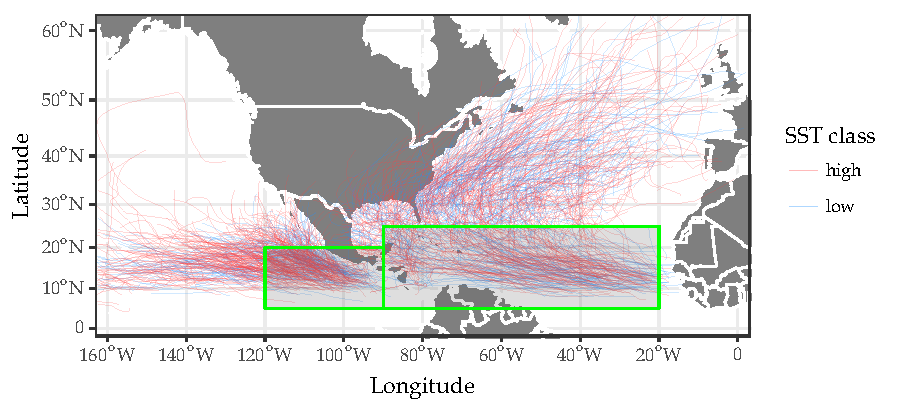
\includegraphics[width=\textwidth]{images/full-map}
	\caption{Tropical-cyclones best tracks for the North Atlantic and Northeast Pacific Oceans}
	\label{fig:full-map}
\end{figure}

%-----------------------------------------------------------------
\subsection{Unified data set}\label{ssec:unified-data-set}
For this study, we have developed a unified data set that summarises the relevant variables of each analysed tropical-cyclone using data from the HURDAT2 and the HadISST1.

In \Cref{hd:unified-dataset-head} one can see the structure of the unified data set to illustrate the variables we use, as well as their data type.
\begin{table}[H]
	\centering
	\ttfamily
	\resizebox{\textwidth}{!}{%
	\begin{tabular}{r r r r r r r r r r r r r}
		\toprule
		\toprule
		storm.id & storm.name & n.obs & storm.duration &    storm.pdi & max.wind & mean.wind & mean.sq.wind & storm.year & basin &   sst & sst.norm & sst.class \\
		<chr>    & <chr>      & <int> &          <dbl> &        <dbl> &    <int> &     <dbl> &        <dbl> &      <int> & <chr> & <dbl> &    <dbl> &     <chr> \\
		\midrule
		AL011966 & ALMA       &    42 &            252 &  34632626747 &      110 &      56.4 &        3750  &       1966 & NATL  &  27.6 &    0.998 &       low \\
		AL021966 & BECKY      &     9 &             54 &   3413930334 &       65 &      46.1 &        2353. &       1966 & NATL  &  27.6 &    0.998 &       low \\
		AL031966 & CELIA      &    36 &            216 &   7839872104 &       70 &      35.4 &        1488. &       1966 & NATL  &  27.6 &    0.998 &       low \\
		AL041966 & DOROTHY    &    37 &            222 &  21340832518 &       75 &      54.9 &        3211. &       1966 & NATL  &  27.6 &    0.998 &       low \\
		AL051966 & ELLA       &    26 &            156 &   4646503652 &       45 &      37.7 &        1487. &       1966 & NATL  &  27.6 &    0.998 &       low \\
		AL061966 & FAITH      &    69 &            414 & 120569417711 &      110 &      79.0 &        6722. &       1966 & NATL  &  27.6 &    0.998 &       low \\
		\bottomrule
	\end{tabular}}
	\caption{Excerpt of the North Atlantic data set}
	\label{hd:unified-dataset-head}
\end{table}

This unified data sets for the North Atlantic and Northeast Pacific basins can be downloaded from the GitLab repository of this project~\cite{o:gitlab-repo} in \texttt{CSV} format.

Alternatively, these data sets have been packaged into an R package called \texttt{HurdatHadISSTData} \cite{o:gitlab-data-repo}, and can be installed using the \texttt{devtools} package:
\begin{lstlisting}
library(devtools)
install_git("https://gitlab.com/aldomann/hurdat-hadisst-data.git")
\end{lstlisting}

The names of these data sets in the \texttt{HurdatHadISSTData} package are:
\begin{itemize}
	\item \texttt{tc.pdi.natl} -- Data set for the North Atlantic basin.
	\item \texttt{tc.pdi.epac} -- Data set for the Northeast Pacific basin.
	\item \texttt{tc.pdi.all} -- Data set for both basins.
\end{itemize}
